\documentclass[main.tex]{subfiles}

\begin{document}

\section{Numerical integration}\label{sec:numerical_integration}

As explained in Section \ref{m-subsec:numerical_integration}, the periods
of the generating cycles $\gamma\in \Gamma$ are expressed in terms of
elementary integrals
\eqref{m-eq:elem_num_int}
\begin{equation*}
    I_{a,b}(i,j) = \int_{-1}^1\frac{u^{i-1}\du}{(1-u^2)^{\frac jm}\ytab(u)^j}
\end{equation*}
where $(a,b)\in E$ and $\omega_{i,j}\in\W$.
We restrict the numerical analysis to this case.

In this section, we denote by $α$ the value $1-j/m$, which is the crucial parameter for numerical integration.
Note that $α=1/2$ for hyperelliptic curves, while for general superelliptic curves $α$ ranges
from $1/m$ to $\frac{m-1}m$ depending on the differential form $\omega_{i,j}$ considered.

We study here two numerical integration schemes which are suitable for arbitrary
precision computations:
\begin{itemize}
    \item
        the double-exponential change of variables is completely general \cite{Molin2010} and its robustness
allows to compute rigorously all integrals of periods in a very unified setting
even with different values of $\alpha$;
\item in the special case of hyperelliptic curves however,
    the Gauss-Chebychev method \cite[25.4.38]{AbramowitzStegun} applies and
    provides a better scheme (fewer and simpler integration points).
\end{itemize}
For $m > 2$, the periods could also be computed using general Gauss-Jacobi integration
of parameters $\alpha,\alpha$. However, a different scheme has to be computed for each $\alpha$
and it now involves computing roots of general Jacobi polynomials to large accuracy, which
makes it hard to compete with the double-exponential scheme.

\begin{rmk}
    Even for hyperelliptic curves it can happen that the double exponential scheme outperforms Gauss-Chebychev on
    particular integrals. This is easy to detect in practice and we can always switch to
    the best method.
\end{rmk}

\subsection{Double-exponential integration}\label{m-subsec:de_int}

Throughout this section, $λ\in[1,\frac{π}2]$ is a fixed parameter.
By default the value $λ=\frac{π}2$ is a good choice, however
smaller values may improve the constants. We will not address
this issue here.
\medskip

Using the double-exponential change of variable
\begin{equation}
    \label{eq:de_change}
u=\tanh(λ\sinh(t)),
\end{equation}
the singularities of \eqref{eq:elem_num_int} at $\pm1$ are pushed to infinity and
the integral becomes
\begin{equation*}
    I_{a,b}(i,j) = \int_\R g(t)\dt
\end{equation*}
with
\begin{equation*}
   g(t) = \frac{u(t)^{i-1}}{\ytab(u(t))^j}\frac{λ\cosh(t)}{\cosh(λ\sinh(t))^{2α}}.
\end{equation*}

Let
\begin{equation*}
    Z_r = \set{\tanh(λ\sinh(z)), -r<\Im(z)<r }
\end{equation*}
be the image of the strip of width $2r$ under the change of
variable \eqref{m-eq:de_change}.

Since we can compute the distance of each point $u_k \in U^+ \cup U^-$ (see \ref{m-eq:uab_image}) to
both $[-1,1]$ and the neighborhood $Z_r$ (see \S \ref{m-subsec:de_case}), we obtain
  \begin{lemma}
      Let $r \in ]0,\frac{\pi}{2}[$ be such that
          $\lambda\sin(r)<\frac{\pi}2$ and
          $(U^+ \cup U^-) \cap Z_r = \varnothing$, then
      $g$ is holomorphic on $\set{-r<\Im(z)<r}$ and
      there exist explicitly computable
      constants $M_1$, $M_2$ such
      that
      \begin{itemize}
          \item $\abs{\frac{u^{i-1}}{\ytab(u)^{j}}}\leq M_1$ for all $u\in[-1,1]$,
          \item $\abs{\frac{u^{i-1}}{\ytab(u)^{j}}}\leq M_2$ for all $u\in Z_r$.
      \end{itemize}
  \end{lemma}

Fixing such a value $r$, we also introduce the following quantities
\begin{equation*}
    \begin{cases}
    X_r &=\cos(r)\sqrt{\frac{π}{2λ\sin r}-1} \\[0.2cm]
    B(r,α) &=
    \frac{2}{\cos r}
    \left(
        \frac{X_r}2\left(\frac1{\cos(λ\sin r)^{2α}}+\frac1{X_r^{2α}}\right)
        +\frac{1}{2α\sinh(X_r)^{2α}}
    \right).
    \end{cases}
\end{equation*}

Once we have computed the two bounds $M_1$, $M_2$ and the constant $B(r,α)$,
we obtain a rigorous integration scheme as follows:
\begin{thm}
    \label{thm:de_int}
    With notation as above, for all $D>0$, choose $h$ and $N$ such that
    \begin{equation}
    \label{eq:de_parameters}
        \begin{cases}
            h \le \frac{2πr}{D + \log(2M_2 B(r,α) + e^{-D})}\\[0.2cm]
            Nh \ge \asinh\left(\frac{D+\log\big(\frac{2^{2α+1}M_1}{α}\big)}{2αλ}\right),
        \end{cases}
    \end{equation}
    then
    \begin{equation*}
        \abs{
            I_{a,b}(i,j)
            - h\sum_{\ell=-N}^N
            w_\ell \frac{u_\ell^{i-1}}{\ytab(u_\ell)^j}
        } \leq e^{-D},
    \end{equation*}
    where
    \begin{equation*}
        \begin{cases}
            u_\ell = \tanh(λ\sinh(\ell h)),\\[0.2cm]
            w_\ell = \frac{λ\cosh(\ell h)}{\cosh(λ\sinh(\ell h))^{2α}}.
        \end{cases}
    \end{equation*}
\end{thm}

The proof follows the same lines as the one in \cite[Thm. 2.10]{Molin2010}:
we write the Poisson formula on $h\Z$ for the function $g$
\begin{equation*}
    \underbrace{h\sum_{\abs{k}>N}g(kh)}_{e_T}
 + h\sum_{k=-N}^N g(kh)
 = \int_\R g(t)\dt
 + \underbrace{\sum_{k\in\Z^\ast} \hat g\left(\frac{k}{h}\right)}_{e_Q}
\end{equation*}
and control both error terms $e_T$ and $e_Q$ by Lemma \ref{m-lem:de_error_trunc}
and \ref{m-lem:de_error_quad} below. The actual parameters $h$ and $N$ follow
from bounding each error by $e^{-D}/2$
(the condition of Lemma \ref{lem:de_error_trunc} being automatically satisfied).

\begin{lemma}[truncation error]
    \label{lem:de_error_trunc}
    For all $N,h$ such that $2αλ\cosh(Nh)>1$ we have
    \begin{equation*}
        \sum_{\abs{k}>N}\abs{hg(kh)}
        \leq \frac{2^{2α} M_1}{α}\exp(-2αλ\sinh(Nh)).
    \end{equation*}
\end{lemma}
\begin{proof}
% (ch/ch(l.sh)^a)' < 0 for sh.ch(l.sh) < a.l.ch^2.sh(l.sh)
% ok for a.l.ch > 1 since th < th(l.sh)
    We bound the sum by an integral (the condition ensures the function
    is decreasing)
    \begin{align*}
        \sum_{\abs{k}>N}\abs{hg(kh)}
        &\leq2M_1\int_{Nh}^\infty\frac{λ\cosh(t)}{\cosh(λ\sinh(t))^{2α}}
        =2M_1\int_{λ\sinh(Nh)}^\infty\frac{\dt}{\cosh(t)^{2α}}\\
        &\leq 2^{2α+1} M_1\int_{λ\sinh(Nh)}^\infty e^{-2αt}\dt
        = \frac{2^{2α} M_1}{α}e^{-2αλ\sinh(Nh)}.
    \end{align*}
\end{proof}

\begin{lemma}[discretization error]
    \label{lem:de_error_quad}
    With the current notations,
    \begin{equation*}
        \sum_{k\neq0}\abs{\hat g\left(\frac kh\right)}
        \leq
        \frac{2M_2B(r,α)}{e^{2πr/h}-1}.
    \end{equation*}
\end{lemma}
\begin{proof}
We first bound the Fourier transform by a shift of contour
\begin{equation*}
    \forall X>0, \hat g(\pm X) = e^{-2πXr} \int_{\R} g(t\mp ir) e^{-2iπtX}\dt
\end{equation*}
so that
\begin{equation*}
    \sum_k \abs{\hat g\left(\frac kh\right)}
    \leq
    \frac{2M_2}{e^{2πr/h}-1}\int_\R \abs{
    \frac{λ\cosh(t+ir)}{\cosh(λ\sinh(t+ir))^{2α}}}\dt.
\end{equation*}

Now the point $λ\sinh(t+ir) = X(t)+iY(t)$ lies on the hyperbola
$Y^2 =λ^2(\sin^2r+\tan^2 rX^2)$, and
\begin{equation*}
    \begin{cases}
    \abs{λ\cosh(t+ir)} &\leq λ\cosh(t) =\frac{X'(t)}{\cos(r)}\\[0.2cm]
    \abs{\cosh(X+iY)}^2 &= \sinh(X)^2+\cos(Y)^2,
    \end{cases}
\end{equation*}
so that
\begin{equation*}
    \int_\R \abs{
    \frac{λ\cosh(t+ir)}{\cosh(λ\sinh(t+ir))^{2α}}}\dt
    \leq
    \frac{2}{\cos r}\int_0^\infty\frac{\d X}{(\sinh(X)^2+\cos(Y)^2)^α}.
\end{equation*}
For $X_0=0$ we get $Y_0=λ\sin r<\frac{π}2$, and $Y_r=\frac{π}2$ for
$X_r=\cos(r)\sqrt{\frac{π}{2Y_0}-1}$.

  We cut the integral at $X=X_r$ and write
  \begin{align*}
      \int_0^{X_r}\frac{\d X}{(\sinh(X)^2+\cos(Y)^2)^α}
      & \leq \int_0^{X_r}\frac{\d X}{(X^2+\cos^2Y)^α} \\
      \int_{X_r}^\infty\frac{\d X}{(\sinh(X)^2+\cos(Y)^2)^α}
      & \leq \int_{X_r}^\infty\frac{\d X}{(\sinh X)^{2α}}.
  \end{align*}

  We bound the first integral by convexity:
  since $Y(X)$ is convex and $\cos$ is concave decreasing for $Y\leq Y_r$ we
  obtain by concavity of the composition
  \begin{equation*}
      \forall X\leq X_r, \cos(Y)\geq \cos(Y_0)\left(1-\frac{X}{X_r}\right).
  \end{equation*}
  Now $X^2+\cos^2Y\geq P_2(X)$ where
  \begin{equation*}
     P_2(X) = \left(1+\frac{\cos^2(Y_0)}{X_r^2}\right)X^2 -2\frac{\cos^2(Y_0)}{X_r}X+\cos^2(Y_0)
  \end{equation*}
  is a convex quadratic, so $X\mapsto P_2(X)^{-α}$ is still convex and the integral
  is bounded by a trapezoid
  \begin{equation*}
  \int_0^{X_r}\frac{\d X}{P_2(X)^α}\leq \frac{X_r}2\left(P_2(0)^{-α}+P_2(X_r)^{-α}\right)
      = \frac{X_r}2\left(\frac1{\cos(Y_0)^{2α}}+\frac1{X_r^{2α}}\right).
  \end{equation*}

  For the second integral we use
  $\sinh(X)\geq\sinh(X_r)e^{X-X_r}$ to obtain
  \begin{equation*}
      \int_{X_r}^\infty \frac{\d X}{\sinh(X)^{2α}} \leq \frac1{2α\sinh(X_r)^{2α}}.
  \end{equation*}
\end{proof}

\subsection{Gauss-Chebychev integration}
\label{subsec:gauss_chebychev_integration}

In the case of hyperelliptic curves, we have $α=\frac12$ (and $j=1$) and the integral
\begin{equation*}
    \int_{-1}^1\frac{\varphi_{i,1}(u)}{\sqrt{1-u^2}}\du
\end{equation*}
can be efficiently handled by Gaussian integration with weight
$1/\sqrt{1-u^2}$,
for which the corresponding orthogonal polynomials are
Chebychev polynomials.

In this case, the integration formula is particularly
simple: there is no need to actually compute the Chebychev polynomials
since their roots are explicitly given as cosine functions \cite[25.4.38]{AbramowitzStegun}.
\begin{thm}[Gauss-Chebychev integration]
    Let $g$ be holomorphic around $[-1,1]$. Then for all
    $N$, there exists $\xi \in ]-1,1[$ such that
    \begin{equation}
        \label{eq:gauss_chebychev}
        \int_{-1}^1\frac{g(u)}{\sqrt{1-u^2}}\du
        - \sum_{\ell=1}^N w_k g(u_\ell)
        = \frac{π2^{2N+1}}{2^{4N}}\frac{g^{(2N)}(\xi)}{(2N)!}
     = E(N),
    \end{equation}
    with constant weights $w_\ell = w =\frac{π}N$
    and nodes $u_\ell = \cos\left(\frac{2\ell-1}{2N}π\right)$.
\end{thm}

Moreover, very nice estimates on the error $E(N)$ can by obtained by applying
the residue theorem on an ellipse $ε_r$ of the form
\begin{equation*}
    ε_r = \set{z \in \C, \abs{z-1}+\abs{z+1} = 2\cosh(r) }.
\end{equation*}

  \begin{figure}[H] \begin{center}
      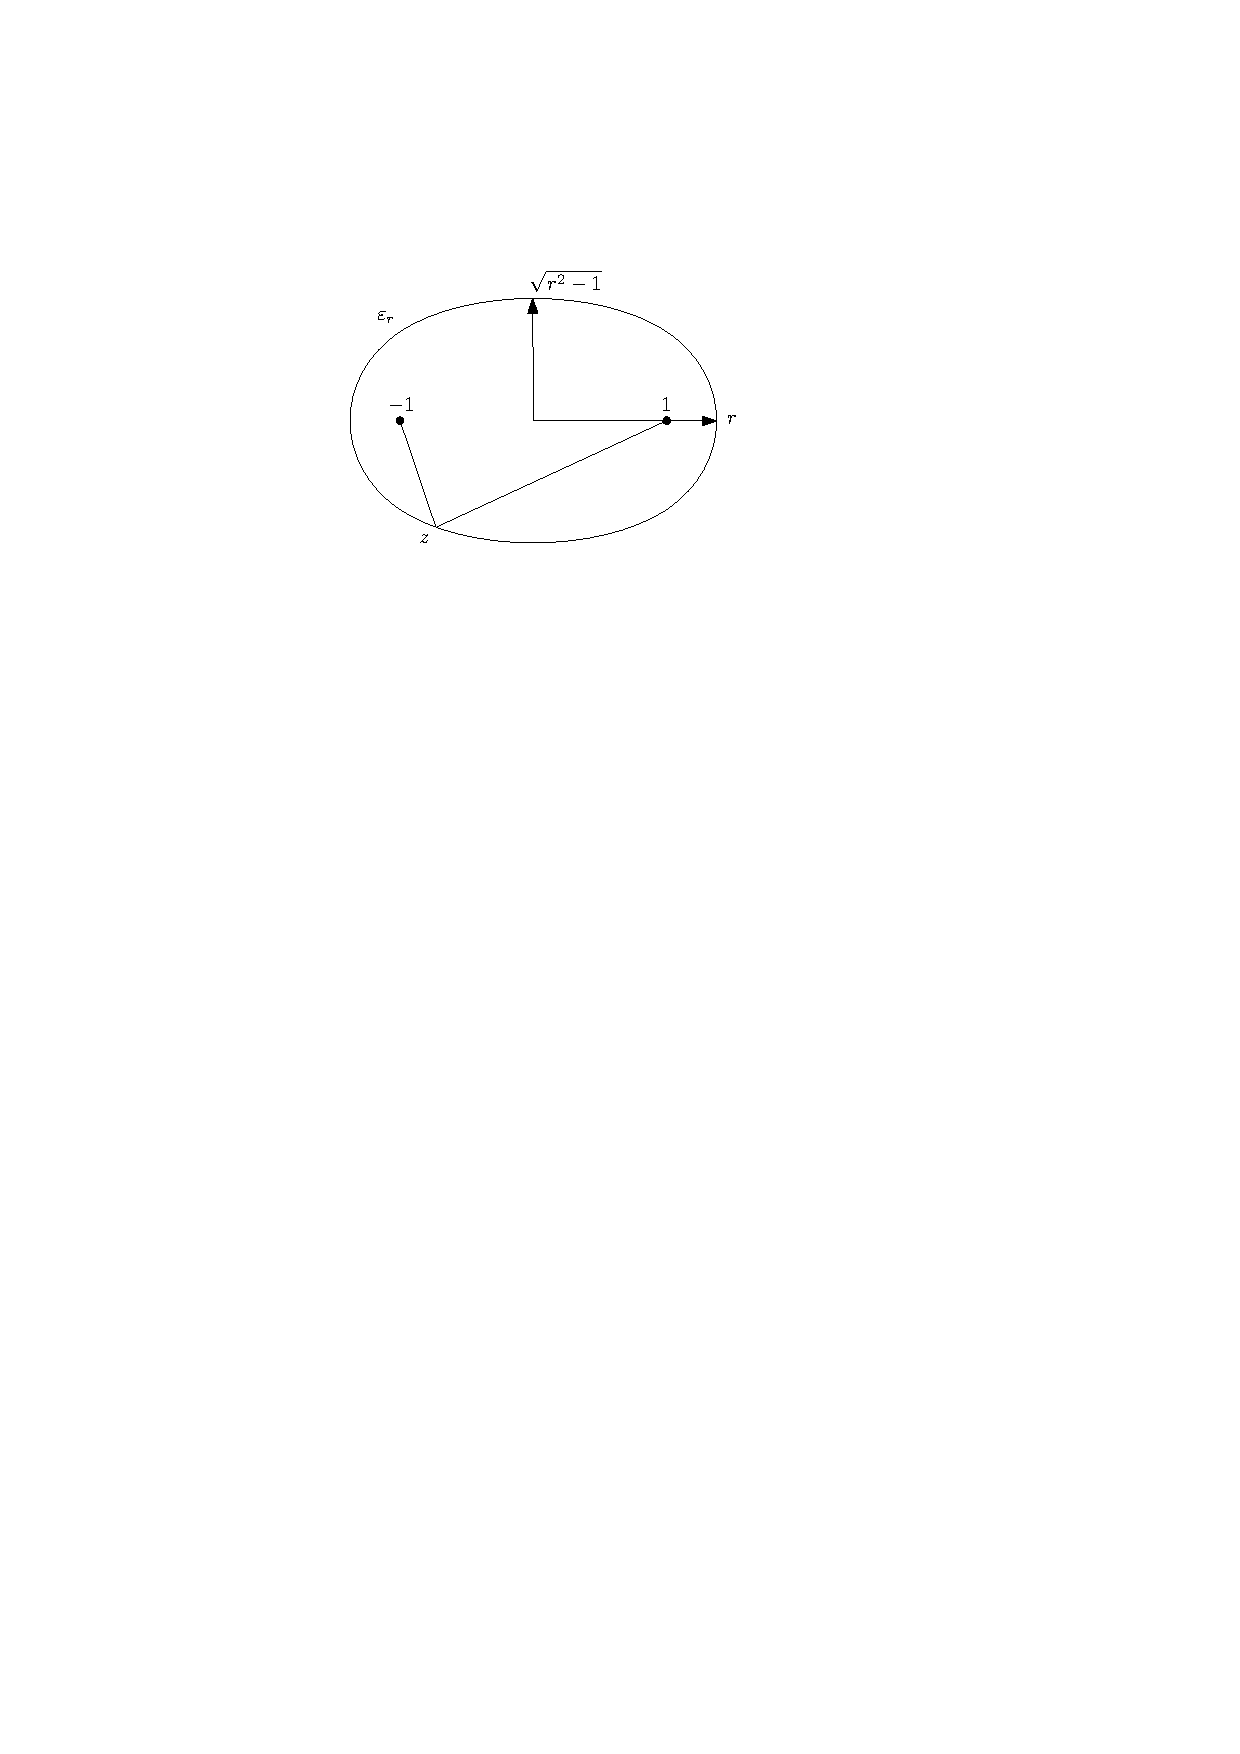
\includegraphics[width=5cm,page=1]{images/ellipse.pdf}
  \end{center} \caption{ellipse parameters.}
  \label{fig:ellipse1} \end{figure}

  \begin{thm}[{\cite[Theorem 5]{ChawlaJain68}}]
    Let $r>0$ such that $g$ is holomorphic on $ε_r$. Then
    the error in \eqref{m-eq:gauss_chebychev} satisfies
    \begin{equation*}
        \abs{E(N)}\leq \frac{2πM(r)}{e^{2rN}-1}
    \end{equation*}
    where $M(r)=\max\set{\abs{g(z)},z\in ε_r}$.
\end{thm}

Now we apply this theorem with a function
$g_{i}(u)=\frac{u^i}{\sqrt{\prod(u-u_k)}}$, so that the error can be explicitly
controlled a priori.

\begin{lemma}
    \label{lem:param_r}
    Let $r>0$ be such that $2\cosh(r)<\abs{u_k-1}+\abs{u_k+1}$ for all
    points $u_k \in U^+ \cup U^-$,
    then there exists an explicitly computable
    constant $M(r)$ such that for all $u\in ε_r$
    \begin{equation*}
        \abs{\frac{u^{i-1}}{\ytab(u)}}\leq M(r).
    \end{equation*}
\end{lemma}
\begin{proof}
We simply compute the distance
        $d_r(u_k) = \inf_{z\in ε_r}\abs{z-u_k}$
 from a point $u_k$ to the ellipse $ε_r$, and let
 $M(r) =  \frac{\cosh(r)^{i-1}}{\sqrt{\prod d_r(u_k)} }$.
 For simplicity, we can use the triangle inequality
 $d_r(u_k)\geq \cosh(r_k)-\cosh(r)$, where
 $2\cosh(r_k)=\abs{u_k-1}+\abs{u_k+1}$.
\end{proof}

\begin{thm}
    \label{thm:gc_int}
    With $r$ and $M(r)$ satisfying Lemma \ref{m-lem:param_r},
    for all $N$ such that
    \begin{equation*}
        \label{eq:Ngc}
        N \geq \frac{D+\log(2πM(r))+1}{2r},
    \end{equation*}
    we have
    \begin{equation*}
        \abs{I_{a,b}(i,1)
        - \frac{π}N\sum_{\ell=1}^N\frac{u_\ell^{i-1}}{\ytab(u_\ell)}}
            \leq e^{-D},
    \end{equation*}
    where $u_\ell=\cos\left(\frac{2\ell-1}{2N}π\right)$.
\end{thm}

More details on the choice of $r$ and the computation of $M(r)$
are given in \S \ref{m-par:gc_int_r}.

\iffalse
the $2n$-th derivative can be
estimated quite precisely by Cauchy formula.

\newcommand{\rmax}{r_{\mathrm{max}}}
\begin{lemma}
    Let $u_i$ be the roots of $Q$, and $r_i$ the distance from
    $u_i$ to $[-1,1]$. Let also $\rmax$ be the minimum of $r_i$.

    Then for all $r<\rmax$,
    \begin{equation}
    \abs{E_n} \leq \frac{2π}rB(r)(2r)^{-2n}
    \end{equation}
    where
    \begin{equation}
        B(r) = \frac1{\prod_i(r_i-r)}
    \end{equation}
\end{lemma}

For fixed $N$, assuming the minimum value $\rmax$ is attained for exactly
$m$ roots $u_i$, we can optimize the choice of $r$ by writing
$r=\rmax(1-λ)$ so that $B(r)\leq\frac{B_1}{(\rmaxλ)^m}$, where
$B_1=\prod(r_i-\rmax)$, the product being on those $r_i>\rmax$.

Then
\begin{equation}
    \frac{2π}rB(r)(2r)^{-2n}
    = \frac{2πB_1}{\rmax^m} λ^{-m}(2\rmax(1-λ))^{-2n-1}
\end{equation}
and $λ^m(1-λ)^{2n+1}$ is maximum for
\begin{equation}
    λ = \frac{m}{2n+1+m}
\end{equation}
in which case
$λ^m(1-λ)^{2n+1}=(1+\frac{2n+1}m)^{-m}(1+\frac{m}{2n+1})^{-(2n+1)}$.

We therefore consider this value of $λ$, so that
\begin{equation}
    E(n) \leq
    \frac{2πB_1}{\rmax^m}
    (1+\frac{2n+1}m)^m(1+\frac{m}{2n+1})^{2n+1}(2\rmax)^{-2n-1}
\end{equation}

  \begin{align}
      \sinh(x+iy) &= \sinh x\cos y+i\cosh x\sin y\\
      \cosh(x+iy) &= \cosh x\cos y+i\sinh x\sin y
  \end{align}
  so that writing $λ\sinh(t+ir)=X+iY$ we express the integral in terms
  of $X,Y$ with
  \begin{align}
      X &= λ\sinh t\cos r\\
      Y &= λ\cosh t\sin r\\
      Y^2 =λ^2(\sin^2r+\tan^2 rX^2)\\
      λ\cosh(t+ir) &= λ\cosh t\cos r+iλ\sinh t\sin r \\
                     &= Y/\tan(r) + i X\tan(r)\\
      \abs{\cosh(X+iY)}^2
      &= \cosh^2 X\cos^2 Y+\sinh^2 X\sin^2 Y \label{eq:boundchcos}\\
      &= \sinh^2 X + \cos^2 Y \label{eq:boundchsh}
  \end{align}
\fi

\iffalse
assume(t,real);
assume(tau,real);
assume(l,real);
assume(l>0);
assume(l<Pi/2);
phi:=tanh(l*sinh(t+I*tau));;
simplify(expand(diff(phi,t$1)));
\fi

\biblio
\end{document}
